\begin{figure*}[!hbtp]
  \centering

  \subfloat{
    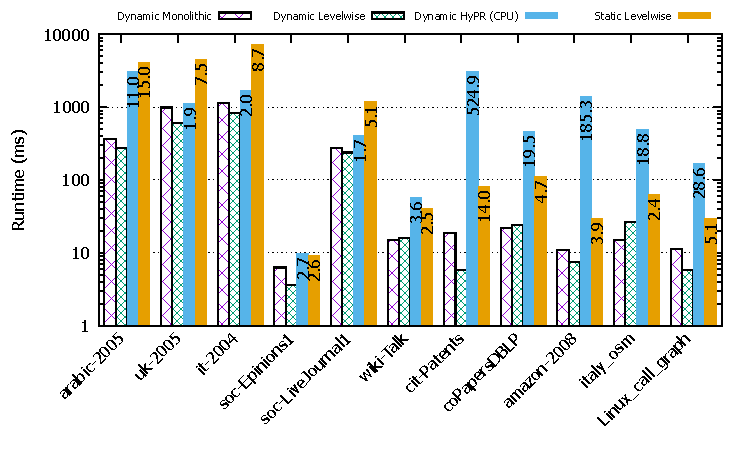
\includegraphics[width=0.48\textwidth]{out/pr-mono-vs-levl-omp-time.pdf}
    \label{fig:pr-mono-vs-levl-omp-time}
  }
  \subfloat{
    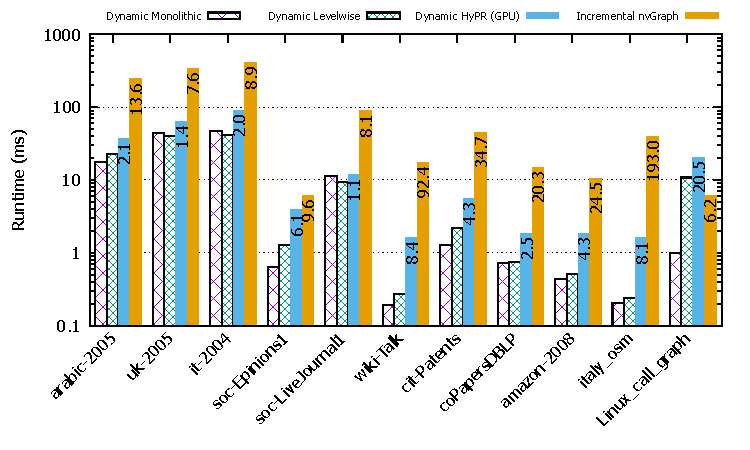
\includegraphics[width=0.48\textwidth]{out/pr-mono-vs-levl-cuda-time.pdf}
    \label{fig:pr-mono-vs-levl-cuda-time}
  }

  \caption{Time taken for PageRank computation with  \monolithicPR{} and \levelwisePR{} for various batch sizes on the CPU (shown on the left) and the GPU (shown on the right). Batch sizes of 500, 1000, 2000, 5000, and 10000 are used. Time taken with \emph{pure CPU implementation of HyPR} and \emph{plain STIC-D PageRank (static Levelwise)} on the CPU, and speedup of \levelwisePR{} over the two approaches (labeled on top of the respective bars) is also included for comparison. Time taken with \emph{pure GPU implementation of HyPR} and \emph{incremental nvGraph PageRank} on the GPU, and speedup of \monolithicPR{} over the two approaches is included as well.}
  \label{fig:pr-mono-vs-levl-time}
\end{figure*}
